\documentclass[11pt]{article}
\usepackage[margin=1in]{geometry}
\usepackage[T1]{fontenc}
\usepackage{lmodern}
\usepackage{microtype}
\usepackage{amsmath}
\usepackage{setspace}
\usepackage{booktabs}
\usepackage{graphicx}
\usepackage{adjustbox}
\usepackage{caption}
\usepackage{float}
\usepackage[round,authoryear]{natbib}
\usepackage[dvipsnames]{xcolor}
\usepackage[colorlinks=true,linkcolor=NavyBlue,citecolor=NavyBlue,urlcolor=NavyBlue]{hyperref}
\captionsetup{font=small,labelfont=bf}
\setstretch{1.25}

% Every number below comes from the replication scripts (output/*/tables/macros_*.tex)
\newcommand{\gapChange}{-26}
\newcommand{\gapNW}{6.1}
\newcommand{\gapPre}{-19}
\newcommand{\nBritCos}{215}
\newcommand{\nBritRec}{258,127}
\newcommand{\nNearCos}{25}
\newcommand{\nNearObs}{1,605}
\newcommand{\nPostCos}{44}
\newcommand{\nPostObs}{3,940}
\newcommand{\nPostSecs}{326}
\newcommand{\nPreCos}{42}
\newcommand{\nPreObs}{1,948}
\newcommand{\nRVcos}{83}
\newcommand{\nRaw}{595,675}
\newcommand{\nReassigned}{20,643}
\newcommand{\relSDelig}{17}

\newcommand{\densP}{0.02}
\newcommand{\didPwb}{0.35}
\newcommand{\didSE}{8.7}
\newcommand{\didTau}{9.6}
\newcommand{\massZero}{4}
\newcommand{\meanSpreadNotElig}{43}
\newcommand{\ordPrw}{0.44}
\newcommand{\ordSE}{40}
\newcommand{\ordTau}{-74}
\newcommand{\preSE}{5.1}
\newcommand{\preTau}{1.0}
\newcommand{\rdCIhi}{25.0}
\newcommand{\rdCIhiHone}{22.9}
\newcommand{\rdCIlo}{-1.6}
\newcommand{\rdCIloHone}{-1.5}
\newcommand{\rdGlHone}{9}
\newcommand{\rdGrHone}{20}
\newcommand{\rdH}{0.76}
\newcommand{\rdNHone}{1,605}
\newcommand{\rdPwbHone}{0.16}
\newcommand{\rdSECY}{7.9}
\newcommand{\rdSEDonut}{5.8}
\newcommand{\rdSEHone}{6.2}
\newcommand{\rdTau}{9.8}
\newcommand{\rdTauCY}{9.1}
\newcommand{\rdTauDonut}{5.1}
\newcommand{\rdTauHone}{10.7}
\newcommand{\sdRelBand}{19}

\newcommand{\agreeAll}{99}
\newcommand{\agreeDated}{99.8}
\newcommand{\agreeNear}{98}
\newcommand{\corrXyld}{0.98}
\newcommand{\feSE}{11.2}
\newcommand{\feTau}{5.0}
\newcommand{\feivF}{56}
\newcommand{\feivSE}{2.3}
\newcommand{\feivTau}{-8.2}
\newcommand{\fsCoef}{0.84}
\newcommand{\fzF}{40}
\newcommand{\fzSE}{6.7}
\newcommand{\fzTau}{8.9}
\newcommand{\nSwitchCo}{5}
\newcommand{\nSwitchIV}{3}
\newcommand{\nSwitchSec}{44}

\newcommand{\belowStake}{2}
\newcommand{\exactNot}{5}
\newcommand{\exactStake}{47}
\newcommand{\logitInt}{2.25}
\newcommand{\lpmInt}{0.32}
\newcommand{\lpmIntSE}{0.17}
\newcommand{\lpmfeInt}{0.96}
\newcommand{\lpmfeIntSE}{0.25}
\newcommand{\nStake}{34}
\newcommand{\placFive}{0.09}
\newcommand{\placFour}{-0.09}
\newcommand{\placTwo}{0.08}
\newcommand{\ppNot}{51}
\newcommand{\ppStake}{93}
\newcommand{\probitInt}{1.24}

\newcommand{\actAnn}{23.0}
\newcommand{\actAnnSE}{10.4}
\newcommand{\actCIHi}{15.3}
\newcommand{\actCILo}{-17.3}
\newcommand{\actMatched}{7.2}
\newcommand{\actMatchedSE}{6.0}
\newcommand{\actNctrl}{13}
\newcommand{\actNtreat}{11}
\newcommand{\actPwb}{0.93}
\newcommand{\actSE}{8.3}
\newcommand{\actTau}{-1.0}
\newcommand{\esLate}{-20}
\newcommand{\esPeak}{37}
\newcommand{\esPre}{6}


\newcommand{\tabnote}[1]{\par\vspace{3pt}\begin{minipage}{\textwidth}\footnotesize\setstretch{1}\textit{Notes:} \input{#1}\end{minipage}}

\title{\textbf{Trustee Status and the Cost of Railway Capital:}\\[2pt]
\large Regulatory Eligibility, Dividend Management, and Bond Prices in Britain, 1879--1922\thanks{Independent research project. Code and data instructions: \url{https://github.com/zeynamalik/trustee-status-railway-finance}. Data: Investors Monthly Manual, International Center for Finance, Yale School of Management. All errors are my own.}}
\author{Zeyna Malik}
\date{November 2026}

\begin{document}
\maketitle

\begin{abstract}
\noindent Under the Trustee Act 1893, British trustees could buy the debenture and preference stock of a railway only if the company had paid at least 3\% on its ordinary stock in each of the previous ten years. I use this rule to ask whether eligibility for a regulated class of investors lowered the cost of infrastructure finance. I rebuild ten-year dividend records for British and Irish railway companies from the \textit{Investors Monthly Manual}, 1869--1929, and combine three designs: a regression discontinuity at the 3\% threshold, a difference-in-discontinuities against the years before the rule existed, and the Railways Act 1921, which granted trustee status by statute to every company in the 1923 amalgamation. Railway boards clearly valued the status: once the rule was in force, companies whose ten-year record was at stake almost never paid just under 3\%, and the probability of paying at least 3\% rose sharply relative to the pre-rule period, with no such pattern at placebo thresholds of 2\%, 4\% or 5\%. Bond prices tell a different story. Senior yields show no discontinuity at the threshold (local linear estimate \rdTauHone{} basis points, 95\% interval [$\rdCIloHone$, $\rdCIhiHone$]), the jump did not become more negative once the rule existed, and statutory eligibility in 1921 did not move yields either. At the margin, the legal list shaped corporate payout decisions without measurably changing what investors paid for the claims it covered.
\end{abstract}

\vspace{6pt}
\noindent\textbf{JEL:} G12, G18, G28, G35, N23, N43 \quad \textbf{Keywords:} regulatory eligibility, trustee investments, regression discontinuity, bunching, railway finance, Investors Monthly Manual

\newpage
\section{Introduction}

Regulators often decide what certain investors may hold. Insurance capital rules, bank liquidity requirements, central-bank collateral schedules and pension-fund mandates all sort securities into eligible and ineligible classes. If constrained investors are a large share of the market, eligibility should raise demand and lower the issuer's cost of capital. If they are not, or if the rule merely codifies what prudent investors would buy anyway, eligibility should not matter at the margin. Which case holds is an empirical question, and the answer matters for how much regulatory lists distort the allocation of capital. It is hard to answer with modern data, because eligibility usually follows credit ratings that also carry information about default risk \citep{KisgenStrahan2010}.

Victorian Britain offers a cleaner setting. Under the Trustee Act 1893, which consolidated reforms begun in 1888--89, a trustee could buy the debenture, rentcharge, guaranteed or preference stock of a British or Irish railway company only if the company had ``during each of the ten years last past\ldots paid a dividend at the rate of not less than three per centum per annum on its ordinary stock.'' The rule is mechanical, public and based on a variable that investors could observe in every monthly issue of the financial press. A railway that paid 3\% for ten years qualified; one that paid $2\tfrac{7}{8}$\% in any one of those years did not. Railways were the largest borrowers on the London market and the most heavily debt-financed sector \citep{GoetzmannRouwenhorst2026}, so the rule touched the main channel through which Britain financed its infrastructure.

I build ten-year dividend records for every British and Irish railway in the \textit{Investors Monthly Manual} (IMM), 1869--1929, and match them to the yields of each company's senior securities. The analysis has two parts. The first asks whether companies behaved as if trustee status were valuable. The second asks whether bond prices confirm that it was.

The first answer is yes. After the rule came into force, companies whose ten-year record was intact almost never paid a dividend just below 3\%: of the \nStake{} company-years with an intact record and a dividend within half a point of the threshold, only \belowStake{} fell below it, and \exactStake\% paid exactly 3\%. A difference-in-differences comparison with 1879--1887, when 3\% had no legal meaning, shows a large increase in the probability of paying at least 3\% when the record was at stake (\lpmInt{} in a linear probability model, \lpmfeInt{} with company fixed effects). The same test at 2\%, 4\% and 5\% finds nothing. Boards managed dividends to keep the status.

The second answer is no. A regression discontinuity at the 3\% threshold finds no fall in the yields of trustee-eligible securities. The point estimates are small and positive, and the 95\% confidence intervals rule out discounts larger than a few basis points, against a typical spread of about \meanSpreadNotElig{} basis points over consols for securities just below the threshold. The discontinuity after 1893 is, if anything, less favorable to eligible securities than in 1879--1887. Estimates by security class, within-security fixed-effects estimates, a fuzzy RD that uses an independently transcribed dividend measure to correct for misclassification, and the 1921 statutory grant of trustee status all point the same way.

These findings contribute to three literatures. First, they add a clean historical test to work on whether regulatory eligibility affects asset prices. That work finds sizable effects when constrained investors dominate demand \citep{KisgenStrahan2010, EllulJotikasthiraLundblad2011, BeckerIvashina2015}. The Victorian rule appears not to have bound at the margin, plausibly because many trust deeds granted wider powers and because trustees concentrated on first-class stocks well above the threshold. Second, they contribute to the history of the London capital market, where trustee status has been studied for colonial government debt \citep{ChavazFlandreau2017} and credited with raising the price of leading railway debentures in the 1890s \citep{ChambersCrafts}. Third, they document bunching at a regulatory threshold in a payout decision rather than in taxable income \citep{Kleven2016}. Firms responded to the rule even though, at the margin, investors did not.

Section~\ref{sec:institutions} describes the trustee rules. Section~\ref{sec:data} describes the data. Section~\ref{sec:strategy} sets out the empirical strategy, Section~\ref{sec:results} reports results, Section~\ref{sec:discussion} discusses interpretation and limitations, and Section~\ref{sec:conclusion} concludes.

\section{Literature Review}

\paragraph{Regulatory eligibility and the cost of capital.} When regulation restricts what investors may hold, prices can move for reasons unrelated to fundamentals. \citet{KisgenStrahan2010} show that when the SEC recognized a new rating agency for regulatory purposes, bond yields moved in the direction of that agency's ratings, implying that regulatory use of ratings affected firms' cost of capital. \citet{EllulJotikasthiraLundblad2011} find that insurers constrained by capital rules sell downgraded bonds at fire-sale prices, and \citet{BeckerIvashina2015} show that insurers reach for yield within regulatory rating categories. In these settings the regulated investors are large relative to the market. The trustee rules let me study a regime in which eligibility was a sharp function of an observable record rather than of a rating, and in which the regulated investors may or may not have been marginal.

\paragraph{Trustee status in Victorian finance.} The best-studied case is colonial government debt. \citet{ChavazFlandreau2017} show that colonial bonds were priced mainly on liquidity, and place the Colonial Stock Acts of 1877 and 1900 (the second of which made qualifying colonial stocks trustee investments) within a deliberate effort to improve it. For railways, \citet{ChambersCrafts} argue that the Trust Investment Acts of 1889 and 1893 created strong demand for domestic railway debentures in the 1890s and pushed the yields of leading companies close to consols. Those companies, however, were far above the 3\% threshold, so the comparison cannot separate trustee status from credit quality. My regression discontinuity compares companies that differ in eligibility but hardly at all in their dividend records.

\paragraph{The IMM and London returns.} \citet{GoetzmannRouwenhorst2026} use the IMM to document a monotonic hierarchy of returns across the capital structure of London-listed firms, 1870--1929, and show that railways were the most leveraged sector, with debentures and preference stock making up three quarters of their capital. \citet{CampbellGrossmanTurner2021} build broad market indices from the same source, and \citet{CoyleTurner2013} trace the British corporate debt market over the long run. This paper uses the IMM's dividend and yield columns at the level of individual securities to study one regulatory feature of that hierarchy.

\paragraph{Methods.} The regression discontinuity follows \citet{LeeLemieux2010} and \citet{CalonicoCattaneoTitiunik2014}. Because the running variable is a dividend rate declared in eighths of a percent, it has mass points \citep{KolesarRothe2018}. Because firms can influence it, I test for manipulation \citep{McCrary2008, CattaneoJanssonMa2020} and report donut estimates \citep{BarrecaLindoWaddell2016}. The comparison with the pre-rule period is a difference-in-discontinuities \citep{GrembiNanniciniTroiano2016}. With few clusters near the threshold, I use wild-cluster bootstrap inference \citep{CameronGelbachMiller2008, Webb2023}, and I correct for testing several outcomes \citep{Holm1979, RomanoWolf2005}. Misclassification of a binary treatment is non-classical measurement error, so instrumenting with a second measure bounds rather than removes the bias \citep{BlackBergerScott2000}.

\section{Institutional Background}\label{sec:institutions}

\paragraph{The trustee rules.} Before 1888, a trustee without express powers could invest trust funds in little beyond government and a few public stocks and mortgages of land. Proposals in 1888 and the Trust Investment Act 1889 widened these powers; in the 1889 debate a peer noted that the previous year's bill had provided for investment in the preference shares of railways that had paid dividends on their ordinary stock for ten years \citep{Hansard1889}. The Trustee Act 1893 consolidated the law, and its text is the rule I study. Section 1(g) authorized investment ``in the debenture or rentcharge, or guaranteed or preference stock of any railway company in Great Britain or Ireland incorporated by special Act of Parliament, and having during each of the ten years last past before the date of investment paid a dividend at the rate of not less than three per centum per annum on its ordinary stock.'' Section 1(h) separately covered the stock of lines leased in perpetuity at a fixed rent to such a company. The Trustee Act 1925 kept the 3\% test.

Three features matter for the design. First, the test applied to the company's \textit{ordinary} dividend but conferred eligibility on its \textit{senior} securities, so the yields I study are not mechanically tied to the running variable. Second, the test was strict: a single year below 3\% removed a company's senior stocks from the list for a decade. Third, the statutory list was a default. A trustee could use it ``unless expressly forbidden by the instrument creating the trust,'' and settlors were free to grant wider powers. As early as 1871, a member of Parliament observed that railway debenture stock was ``almost invariably included in modern settlements'' \citep{Hansard1871}. If enough trust money already had express power to buy railway stock, the statutory test may have been slack.

\paragraph{War, control and amalgamation.} From August 1914 to August 1921 the railways were under government control, with net revenue guaranteed at 1913 levels. The Ministry of Transport's White Paper of June 1920 \citep{Cmd787} proposed grouping the companies, and the Railways Act 1921 (royal assent 19 August 1921) merged some 120 companies into four on 1 January 1923. Section 15 deemed each amalgamated company to have paid at least 3\% on its ordinary stock in each of the ten years before amalgamation. Holders of senior stock in constituent companies that had failed the test were therefore promised trustee-eligible paper. Holders in companies that already qualified were not. In 1939 a member asked whether a railway might draw on reserves to pay a token dividend on its preferred ordinary stock in order to keep its prior charges on the trustee list \citep{Hansard1939}. Contemporaries plainly saw the status as something boards would pay to protect.

\section{Data}\label{sec:data}

\paragraph{Source.} The IMM, a monthly supplement to \textit{The Economist}, printed for each listed security its description, nominal capital, monthly prices, the editors' ``yield on investment,'' and the rates and dates of the last four dividend payments. The digitized railway file has \nRaw{} security-month records, 1869--1929. I keep the \nBritRec{} records of \nBritCos{} companies located in Great Britain or Ireland, dropping London-registered foreign lines and companies listed mainly under foreign headings.

\paragraph{Classifying securities.} I classify each security in each month from its printed description: debenture, rentcharge, guaranteed, preference, ordinary, preferred or deferred ordinary, or leased line. Ditto lines (``Do do'') inherit the type of the line above. Companies are identified from the harmonized names in the ICF's cleaned file. Because a few names place a security under the wrong company, each page block, whose securities share one printed heading line, takes the majority company. This reassigns \nReassigned{} records, mostly guaranteed sub-line stocks that belong to the lessee whose obligation they are. I hand-code a list of companies that are leased, jointly owned or worked under a guarantee. Their senior stocks qualified, if at all, under s.1(h) rather than the dividend test, so they are excluded (\texttt{config/company\_exclusions.csv}).

\paragraph{The running variable.} For each company and year I take the dividend on its undivided ordinary stock. The IMM prints the last four payments, so the two most recent slots in the latest autumn or December issue are the payments made during the year. Their average is the annual rate. Several large companies split their ordinary stock one-for-one into preferred and deferred halves in the 1890s; for those years the undivided rate is the sum of the two, which matches the undivided quotation where both are printed. The running variable is
\begin{equation}
X_{ct} = \min\{D_{c,t-10}, \ldots, D_{c,t-1}\} - 3,
\end{equation}
computed when at least eight of the ten years are observed. Senior securities are eligible in year $t$ if $X_{ct} \ge 0$. I build two further measures of $D_{ct}$. The first averages dated payments by calendar year. It reuses the printed rates, so it agrees with the slot measure on eligibility in \agreeDated\% of company-years and is only a consistency check. The second divides the IMM's own printed yield by the price, rounded to the nearest eighth. The yield column was transcribed separately from the dividend columns, so this measure carries independent error. It agrees with the slot measure in \agreeAll\% of company-years overall and \agreeNear\% within one point of the threshold. Figure~\ref{fig:histories} shows the dividend record and eligibility of six companies.

\paragraph{Outcome.} The outcome is the current yield of each senior security: the IMM's printed yield, or coupon divided by price where it is missing. The cleaned file has no government bond prices for 1908--1914, so I measure each yield relative to the median yield of all British senior railway securities in the same month, in basis points. This is equivalent to absorbing month fixed effects. All regressions also include year fixed effects. Most railway debenture and preference stock was perpetual, so current yield is close to yield to maturity. Security-years with at least three monthly yields form the panel.

\paragraph{Samples.} Table~\ref{tab:flow} traces the sample. The main sample covers 1894--1913, after the 1893 consolidation and before wartime control, and has \nPostObs{} senior security-years from \nPostCos{} companies. Of these, \nNearObs{} lie within one point of the threshold, from \nNearCos{} companies. The placebo sample covers 1879--1887 and has \nPreObs{} security-years from \nPreCos{} companies. Table~\ref{tab:summary} compares eligible and ineligible securities. Across the full sample, eligible securities belong to larger companies with higher dividends, and their yields are lower and much less dispersed. Near the threshold, those differences narrow sharply.

\section{Empirical Strategy}\label{sec:strategy}

\paragraph{Dividend management.} If boards valued eligibility, a company whose last nine dividends were all at least 3\% faces a cliff: paying $2\tfrac{7}{8}$\% this year removes its senior stocks from the list for ten years. Among company-years with $D_{ct}$ within half a point of 3, I estimate
\begin{equation}\label{eq:bunch}
\Pr(D_{ct} \ge 3) = F\big(\alpha + \beta_1 \text{AtStake}_{ct} + \beta_2 \text{Post}_t + \beta_3 \text{AtStake}_{ct}\times\text{Post}_t + \gamma D_{c,t-1}\big),
\end{equation}
by linear probability, logit and probit, where AtStake means the previous nine dividends were all at least 3\% and Post covers 1894--1913. Dividend persistence \citep{Lintner1956} would make $\beta_1$ positive in both regimes. The interaction $\beta_3$ measures the additional pull toward 3\% once the threshold carries legal weight. Repeating the test at 2\%, 4\% and 5\%, where there was no rule, separates the effect of the rule from round-number smoothing.

\paragraph{Regression discontinuity.} For senior security $i$ of company $c$ in year $t$,
\begin{equation}\label{eq:rd}
y_{ict} = \tau\,\mathbf{1}[X_{ct} \ge 0] + \beta_1 X_{ct} + \beta_2 X_{ct}\,\mathbf{1}[X_{ct} \ge 0] + \delta_t + \kappa_{k(i)} + \varepsilon_{ict}, \quad |X_{ct}| \le h,
\end{equation}
where $\delta_t$ are year effects and $\kappa_k$ are security-class effects. $\tau$ is the effect of eligibility on yields for companies at the threshold. Identification requires that companies just above and just below the threshold are otherwise comparable. Dividend management threatens that assumption, because companies that stretch to pay exactly 3\% may differ from those that do not. I therefore test the density of $X$, check balance in pre-determined characteristics, and report donut estimates that drop company-years at exactly $X=0$. I estimate (\ref{eq:rd}) with \texttt{rdrobust}, which uses MSE-optimal bandwidths and robust bias-corrected intervals, and by OLS within fixed bandwidths. Standard errors are clustered by company. With only \rdGlHone{} companies just below the threshold, I report wild-cluster bootstrap $p$-values with Webb weights. Estimating (\ref{eq:rd}) on 1879--1887, when no rule existed, gives a placebo, and pooling the two regimes gives a difference-in-discontinuities.

\paragraph{Panel and measurement error.} Companies cross the threshold over time, so security fixed effects can identify $\tau$ from changes within a security. Misclassified eligibility attenuates every estimate, so I also estimate a fuzzy RD in which the yield-implied running variable instruments the slot-based treatment. Because the two measures' errors are independent, this corrects much of the attenuation.

\paragraph{The 1921 Act.} For the monthly senior yields of British companies amalgamated in 1923,
\begin{equation}\label{eq:did}
y_{im} = \beta\,\text{Treat}_c \times \text{Post}_m + \alpha_i + \lambda_m + \varepsilon_{im},
\end{equation}
where Treat marks companies that failed the 3\% test in 1921 and Post begins at royal assent. An event study by quarter, relative to 1920Q2, shows the dynamics around the White Paper and the Act. Because the Act also pooled weak and strong companies, $\beta$ combines trustee status with any credit effect of amalgamation, which makes it, if anything, an upper bound on the effect of status alone.

\section{Results}\label{sec:results}

\subsection{Railways managed dividends to keep trustee status}

Figure~\ref{fig:bunching} shows annual ordinary dividends between 1.5\% and 5\% by regime and by whether the record was at stake. Before the rule, companies with an intact record were spread across the range above 3\%. After it, they pile into the bin from 3.00 to 3.25\% and almost never appear just below. Among company-years with a record at stake and a dividend within half a point of the threshold, \exactStake\% paid exactly 3\%, compared with \exactNot\% of companies with no record to protect.

Table~\ref{tab:divmgmt} formalizes the comparison. The interaction in (\ref{eq:bunch}) is \lpmInt{} (s.e.\ \lpmIntSE) in the linear probability model and \lpmfeInt{} (s.e.\ \lpmfeIntSE) with company fixed effects. Logit and probit estimates are \logitInt{} and \probitInt{}. The logit implies that after 1893 a company with its record at stake paid at least 3\% with probability \ppStake\%, compared with \ppNot\% for an otherwise similar company with nothing at stake. The placebo interactions at 2\%, 4\% and 5\% are \placTwo{}, $\placFour$ and \placFive{}, all small and insignificant. Ordinary dividend persistence does not explain the pattern; the legal threshold does.

The bunching also appears in the running variable. Figure~\ref{fig:rv} shows a spike at exactly $X = 0$, which holds \massZero\% of post-1893 company-years. A test of continuity of the density rejects at $p = \densP$ (Table~\ref{tab:validity}, Panel B). This confirms the behavioral response and warns that companies at exactly zero may be selected.

\subsection{Eligibility did not lower senior yields}

Figure~\ref{fig:rd} plots senior yields, net of year and class effects, against $X$. Yields fall smoothly with the strength of the dividend record, with no downward jump at the threshold after 1893 or before 1888. Table~\ref{tab:rd} reports the estimates. The \texttt{rdrobust} estimate is \rdTau{} basis points with a robust 95\% interval of [$\rdCIlo$, $\rdCIhi$] at an MSE-optimal bandwidth of \rdH{} points. Local linear estimates at bandwidths of 0.5, 1 and 1.5 points are all small and positive. At $h = 1$ the estimate is \rdTauHone{} (s.e.\ \rdSEHone, wild-bootstrap $p = \rdPwbHone$), with a 95\% interval of [$\rdCIloHone$, $\rdCIhiHone$]. Dropping the company-years bunched at exactly 3.00\% gives \rdTauDonut{} (s.e.\ \rdSEDonut), and collapsing to one capital-weighted observation per company-year gives \rdTauCY{} (s.e.\ \rdSECY). No specification yields the negative sign that higher demand would imply, and the intervals exclude discounts larger than a few basis points. That is small next to the roughly \meanSpreadNotElig-basis-point spread over consols paid by securities just below the threshold, and next to the \sdRelBand-basis-point standard deviation of relative yields within one point of it.

\subsection{Validity}

Table~\ref{tab:validity} collects the checks. Panel A shows no significant discontinuities in coupon, nominal amount, Irish location or the mix of debentures and preference stock at conventional bootstrap levels. Companies just above the threshold have somewhat smaller ordinary capital, but the difference is imprecise. Panel B reports the density test discussed above. Because the donut estimate is close to the main one, the selected companies at exactly 3\% do not drive the result. Panel C moves the threshold to placebo values on either side and finds estimates of similar size, scattered around zero; Figure~\ref{fig:placebo} extends this to a grid. Panel D estimates the discontinuity before the rule existed: \preTau{} (s.e.\ \preSE). The difference-in-discontinuities, the change in the jump once the rule took effect, is \didTau{} (s.e.\ \didSE, wild-bootstrap $p = \didPwb$), with the wrong sign for a demand effect. Figure~\ref{fig:bandwidth} shows that the estimate is stable across bandwidths from 0.5 to 2 points.

\subsection{By security class, panel and IV estimates}

Table~\ref{tab:byclass} estimates the discontinuity separately for debentures and rentcharges, preference stock and guaranteed stock, with ordinary stock as a placebo. No senior class shows a significant discount after Holm or Romano--Wolf corrections for testing four outcomes. Ordinary stock shows a negative but imprecise jump of $\ordTau$ basis points (s.e.\ \ordSE, Romano--Wolf $p = \ordPrw$). It is not trustee-eligible, and its yield is mechanically tied to the dividend that defines $X$, so this is not evidence of a demand effect.

Table~\ref{tab:paneliv} turns to within-security variation. Only \nSwitchCo{} companies change eligibility between 1894 and 1913, so the fixed-effects estimates are imprecise. With dividend controls the estimate is \feTau{} (s.e.\ \feSE). The fuzzy RD has a strong first stage (coefficient \fsCoef, $F = \fzF$) and a second-stage estimate of \fzTau{} (s.e.\ \fzSE), close to the reduced-form RD. Misclassification does not hide a large effect. The fixed-effects IV in column (6) is negative, but it is identified from \nSwitchIV{} switching companies and should not be read as evidence either way.

\subsection{Trustee status by statute: the Railways Act 1921}

Table~\ref{tab:act} reports the difference-in-differences for the \actNtreat{} amalgamated companies that gained trustee status only through s.15 of the 1921 Act, against \actNctrl{} that already qualified. After royal assent the treated companies' senior yields moved by $\actTau$ basis points relative to controls (s.e.\ \actSE, wild-bootstrap $p = \actPwb$; 95\% interval [$\actCILo$, $\actCIHi$]). Matching each treated security to the control with the closest 1919 yield gives \actMatched{} (s.e.\ \actMatchedSE). Figure~\ref{fig:event} shows the dynamics. Pre-trends are flat through mid-1920. Between the White Paper and royal assent, treated yields rose relative to controls, peaking at about \esPeak{} basis points (Table~\ref{tab:act}, column 2: \actAnn{}, s.e.\ \actAnnSE). By late 1922, as conversion into the new companies' stock approached, they had fallen to about $\esLate$ basis points relative to 1920Q2. The rise coincides with uncertainty over compensation and grouping terms and with the national coal stoppage of April--June 1921. The late decline coincides with the settlement of exchange terms. Neither can be attributed to trustee status alone, and the average effect is close to zero.

\subsection{The descriptive yield gap}

Figure~\ref{fig:gap} plots the average relative yield of eligible and ineligible companies' senior securities. Eligible securities yielded about $\gapPre$ basis points less than ineligible ones before 1888, and the gap widened by a further $\gapChange$ basis points after 1893 (Newey--West s.e.\ \gapNW; Table~\ref{tab:gapnw}). Read naively, this matches the view that trustee status lowered the cost of capital for eligible companies. But eligible companies were larger and had stronger dividend records, and the companies near the threshold, where those differences vanish, show no gap. The widening is better explained by the continued divergence between strong and weak lines than by the rule.

\section{Discussion}\label{sec:discussion}

Why would boards protect a status that bond investors did not price at the margin? Four explanations fit the evidence. First, eligibility was necessary but not sufficient for trustee demand. Prudent trustees concentrated on first-class stocks far above the threshold; in 1938 a member of Parliament complained that the statutory test admitted ``indifferent investments, such as preference shares in some of the railways'' \citep{Hansard1938}. Second, many settlements granted wider powers, so the statutory list may have bound only a small share of trust money. Third, trustee status may have mattered most when raising new capital, through access to the primary market, rather than for the secondary-market yields observed here. Fourth, a dividend of 3\% may have served as a signal in its own right, so that cutting below it conveyed bad news whatever its legal consequences. The data cannot separate these explanations, but all of them imply that firms responded to the rule more than the market did.

The modern parallel is direct. Eligibility rules for insurers, banks and central-bank collateral affect prices when the constrained investors are large relative to the market and the rule binds \citep{KisgenStrahan2010, EllulJotikasthiraLundblad2011}. The Victorian evidence shows the other case: a widely watched list that changed corporate behavior without moving prices at the margin. Whether a regulatory list matters for the cost of capital depends less on its existence than on how much demand it actually constrains.

\paragraph{Limitations.} First, there are few companies near the threshold, so I rely on wild-bootstrap inference and cannot rule out moderate effects for individual security classes. Second, the outcome is a current yield measured relative to the railway market. This is appropriate for perpetual stock but ignores call features. Third, the running variable is built from transcribed dividends. The yield-based instrument addresses independent transcription error but not errors common to both measures, such as the treatment of split stock. Fourth, the hand-coded exclusions of leased and jointly owned lines involve judgment; the list is in the repository and can be varied.

\section{Conclusion}\label{sec:conclusion}

British trust law tied the eligibility of a railway's senior securities to a strict ten-year record of 3\% dividends on its ordinary stock. Railways responded: once the rule was in force, companies with a record to protect bunched their dividends at exactly 3\%. Bond investors did not: at the threshold, eligibility did not lower senior yields, the discontinuity did not become more negative once the rule existed, and the statutory grant of trustee status in 1921 had no measurable effect on average. Regulatory lists can shape corporate decisions without shaping prices, and studying both responses together is necessary to judge what such rules achieve.

\newpage
\setstretch{1}
\begin{thebibliography}{99}\small

\bibitem[Barreca et~al.(2016)]{BarrecaLindoWaddell2016}
Barreca, A.~I., J.~M. Lindo, and G.~R. Waddell (2016). Heaping-induced bias in regression-discontinuity designs. \textit{Economic Inquiry} 54(1), 268--293.

\bibitem[Becker and Ivashina(2015)]{BeckerIvashina2015}
Becker, B. and V.~Ivashina (2015). Reaching for yield in the bond market. \textit{Journal of Finance} 70(5), 1863--1902.

\bibitem[Black et~al.(2000)]{BlackBergerScott2000}
Black, D.~A., M.~C. Berger, and F.~A. Scott (2000). Bounding parameter estimates with nonclassical measurement error. \textit{Journal of the American Statistical Association} 95(451), 739--748.

\bibitem[Calonico et~al.(2014)]{CalonicoCattaneoTitiunik2014}
Calonico, S., M.~D. Cattaneo, and R.~Titiunik (2014). Robust nonparametric confidence intervals for regression-discontinuity designs. \textit{Econometrica} 82(6), 2295--2326.

\bibitem[Cameron et~al.(2008)]{CameronGelbachMiller2008}
Cameron, A.~C., J.~B. Gelbach, and D.~L. Miller (2008). Bootstrap-based improvements for inference with clustered errors. \textit{Review of Economics and Statistics} 90(3), 414--427.

\bibitem[Campbell et~al.(2021)]{CampbellGrossmanTurner2021}
Campbell, G., R.~S. Grossman, and J.~D. Turner (2021). Before the cult of equity: The British stock market, 1829--1929. \textit{European Review of Economic History} 25(4), 645--679.

\bibitem[Cattaneo et~al.(2020)]{CattaneoJanssonMa2020}
Cattaneo, M.~D., M.~Jansson, and X.~Ma (2020). Simple local polynomial density estimators. \textit{Journal of the American Statistical Association} 115(531), 1449--1455.

\bibitem[Chambers and Crafts(n.d.)]{ChambersCrafts}
Chambers, D. and N.~Crafts (n.d.). Late Victorian railways and investor returns. Unpublished manuscript, \url{https://personal.lse.ac.uk/colvinc/clio/chambers-crafts.pdf}.

\bibitem[Chavaz and Flandreau(2017)]{ChavazFlandreau2017}
Chavaz, M. and M.~Flandreau (2017). ``High \& dry'': The liquidity and credit of colonial and foreign government debt and the London Stock Exchange (1880--1910). \textit{Journal of Economic History} 77(3), 653--691.

\bibitem[Cmd. 787(1920)]{Cmd787}
Ministry of Transport (1920). \textit{Outline of Proposals as to the Future Organisation of Transport Undertakings in Great Britain and their Relation to the State}. Cmd. 787. London: HMSO.

\bibitem[Coyle and Turner(2013)]{CoyleTurner2013}
Coyle, C. and J.~D. Turner (2013). Law, politics, and financial development: The great reversal of the UK corporate debt market. \textit{Journal of Economic History} 73(3), 809--845.

\bibitem[Ellul et~al.(2011)]{EllulJotikasthiraLundblad2011}
Ellul, A., C.~Jotikasthira, and C.~T. Lundblad (2011). Regulatory pressure and fire sales in the corporate bond market. \textit{Journal of Financial Economics} 101(3), 596--620.

\bibitem[Goetzmann and Rouwenhorst(2026)]{GoetzmannRouwenhorst2026}
Goetzmann, W.~N. and K.~G. Rouwenhorst (2026). Capital structure, seniority, and risk premia: Evidence from the London Stock Exchange, 1870--1929. NBER Working Paper 34899.

\bibitem[Grembi et~al.(2016)]{GrembiNanniciniTroiano2016}
Grembi, V., T.~Nannicini, and U.~Troiano (2016). Do fiscal rules matter? \textit{American Economic Journal: Applied Economics} 8(3), 1--30.

\bibitem[Hansard(1871)]{Hansard1871}
Hansard (1871). House of Commons debate, 9 May 1871, vol.~206, cols.~575--577.

\bibitem[Hansard(1889)]{Hansard1889}
Hansard (1889). House of Lords debate on the Trust Funds Investment Bill, second reading, 18 July 1889, vol.~338, cols.~663--665.

\bibitem[Hansard(1938)]{Hansard1938}
Hansard (1938). House of Commons, Trustee Act, 21 June 1938.

\bibitem[Hansard(1939)]{Hansard1939}
Hansard (1939). House of Commons written answers, Trustee Acts (railway stocks), 26 July 1939.

\bibitem[Holm(1979)]{Holm1979}
Holm, S. (1979). A simple sequentially rejective multiple test procedure. \textit{Scandinavian Journal of Statistics} 6(2), 65--70.

\bibitem[Kisgen and Strahan(2010)]{KisgenStrahan2010}
Kisgen, D.~J. and P.~E. Strahan (2010). Do regulations based on credit ratings affect a firm's cost of capital? \textit{Review of Financial Studies} 23(12), 4324--4347.

\bibitem[Kleven(2016)]{Kleven2016}
Kleven, H.~J. (2016). Bunching. \textit{Annual Review of Economics} 8, 435--464.

\bibitem[Koles{\'a}r and Rothe(2018)]{KolesarRothe2018}
Koles{\'a}r, M. and C.~Rothe (2018). Inference in regression discontinuity designs with a discrete running variable. \textit{American Economic Review} 108(8), 2277--2304.

\bibitem[Lee and Lemieux(2010)]{LeeLemieux2010}
Lee, D.~S. and T.~Lemieux (2010). Regression discontinuity designs in economics. \textit{Journal of Economic Literature} 48(2), 281--355.

\bibitem[Lintner(1956)]{Lintner1956}
Lintner, J. (1956). Distribution of incomes of corporations among dividends, retained earnings, and taxes. \textit{American Economic Review} 46(2), 97--113.

\bibitem[McCrary(2008)]{McCrary2008}
McCrary, J. (2008). Manipulation of the running variable in the regression discontinuity design: A density test. \textit{Journal of Econometrics} 142(2), 698--714.

\bibitem[Romano and Wolf(2005)]{RomanoWolf2005}
Romano, J.~P. and M.~Wolf (2005). Stepwise multiple testing as formalized data snooping. \textit{Econometrica} 73(4), 1237--1282.

\bibitem[Webb(2023)]{Webb2023}
Webb, M.~D. (2023). Reworking wild bootstrap-based inference for clustered errors. \textit{Canadian Journal of Economics} 56(3), 839--858.

\end{thebibliography}

\noindent\textbf{Statutes.} Trust Investment Act 1889 (52 \& 53 Vict. c.~32); Trustee Act 1893 (56 \& 57 Vict. c.~53), s.~1(g)--(h); Railways Act 1921 (11 \& 12 Geo.~5 c.~55), s.~15; Trustee Act 1925 (15 \& 16 Geo.~5 c.~19).

% ============================================================================
% TABLES
% ============================================================================
\newpage
\setstretch{1}

\begin{table}[p]\centering
\caption{Sample construction}\label{tab:flow}
\begin{tabular}{lrr}
\toprule
Sample restriction & Observations & Companies \\
\midrule
IMM railway security-months, 1869-1929 & 595,675 &  \\
British and Irish railway security-months & 258,127 & 215 \\
Security-years (all security types) & 22,598 &  \\
Senior railway security-years (all years) & 16,776 & 149 \\
\quad with a yield in at least 3 months & 12,265 & 119 \\
\quad company not foreign, leased or jointly owned & 11,086 & 73 \\
\quad ten-year dividend record observed & 9,276 & 60 \\
\quad in 1879-1887 or 1894-1913 & 5,888 & 55 \\
\quad post-1893 regime (main RD sample) & 3,940 & 44 \\
\quad pre-1888 regime (placebo sample) & 1,948 & 42 \\
\bottomrule
\end{tabular}

\tabnote{../output/exhibits/tables/table1_sample_flow_notes.tex}
\end{table}

\begin{table}[p]\centering
\caption{Summary statistics, senior railway securities, 1894--1913}\label{tab:summary}
\adjustbox{max width=\textwidth}{\begin{tabular}{lccccc}
\toprule
 & All & Eligible & Not eligible & Eligible, |X|$\le$1 & Not eligible, |X|$\le$1 \\
\midrule
Current yield (\%) & 3.56 & 3.36 & 3.76 & 3.38 & 3.43 \\
Yield relative to market (bp) & 13.0 & -9.4 & 35.7 & -7.2 & 3.9 \\
\quad (standard deviation) & 102.1 & 17.4 & 140.2 & 18.5 & 19.3 \\
Coupon / fixed dividend (\%) & 4.10 & 4.08 & 4.12 & 4.10 & 3.94 \\
Nominal amount (GBP m) & 3.15 & 4.81 & 1.46 & 3.41 & 1.94 \\
Share debenture or rentcharge & 0.40 & 0.43 & 0.37 & 0.43 & 0.37 \\
Share preference & 0.47 & 0.42 & 0.53 & 0.42 & 0.54 \\
Share guaranteed & 0.12 & 0.15 & 0.09 & 0.15 & 0.10 \\
Irish company & 0.11 & 0.15 & 0.08 & 0.15 & 0.02 \\
Ordinary dividend, year $t-1$ (\%) & 3.45 & 4.93 & 1.94 & 4.26 & 3.07 \\
Ten-year minimum dividend (\%) & 2.48 & 4.14 & 0.80 & 3.47 & 2.40 \\
Security-years & 3,940 & 1,984 & 1,956 & 1,239 & 366 \\
Securities & 326 & 173 & 197 & 145 & 68 \\
Companies & 44 & 25 & 24 & 20 & 9 \\
\bottomrule
\end{tabular}
}
\tabnote{../output/exhibits/tables/table2_summary_stats_notes.tex}
\end{table}

\begin{table}[p]\centering
\caption{Dividend management at the 3\% threshold}\label{tab:divmgmt}
\adjustbox{max width=\textwidth}{\begin{tabular}{lccccccc}
\toprule
 & (1) & (2) & (3) & (4) & (5) & (6) & (7) \\
\midrule
At stake $\times$ post-1893 & 0.321$^{*}$ & 0.958$^{***}$ & 2.248$^{***}$ & 1.245$^{**}$ & 0.078 & -0.090 & 0.091 \\
 & (0.168) & (0.251) & (0.826) & (0.486) & (0.277) & (0.162) & (0.216) \\
At stake & 0.054 & -0.407$^{*}$ & 0.232 & 0.161 & 0.096 & 0.289$^{***}$ & -0.073 \\
 & (0.183) & (0.222) & (0.905) & (0.546) & (0.208) & (0.100) & (0.176) \\
Post-1893 & -0.043 & -0.560$^{***}$ & -0.181 & -0.122 & -0.118 & -0.140 & -0.002 \\
 & (0.121) & (0.162) & (0.515) & (0.321) & (0.143) & (0.125) & (0.102) \\
Dividend in $t-1$ & 0.149$^{***}$ & 0.153$^{***}$ & 0.722$^{**}$ & 0.435$^{**}$ & 0.074 & 0.003 & 0.222$^{***}$ \\
 & (0.050) & (0.046) & (0.290) & (0.171) & (0.077) & (0.053) & (0.070) \\
Threshold $k$ (\%) & 3 & 3 & 3 & 3 & 2 & 4 & 5 \\
Estimator & LPM & LPM & Logit & Probit & LPM & LPM & LPM \\
Company fixed effects & No & Yes & No & No & No & No & No \\
Company-years & 148 & 144 & 148 & 148 & 89 & 174 & 171 \\
Companies & 31 & 31 & 31 & 31 & 23 & 32 & 28 \\
\bottomrule
\end{tabular}
}
\tabnote{../output/results/tables/table7_dividend_management_notes.tex}
\end{table}

\begin{table}[p]\centering
\caption{Trustee eligibility and senior yields: regression-discontinuity estimates}\label{tab:rd}
\adjustbox{max width=\textwidth}{\begin{tabular}{lcccccc}
\toprule
 & (1) rdrobust & (2) & (3) & (4) & (5) & (6) \\
\midrule
Trustee eligible & 9.8 & 5.5 & 10.7 & 5.4 & 5.1 & 9.1 \\
 & (6.8) & (7.2) & (6.2) & (5.1) & (5.8) & (7.9) \\
$p$-value & 0.085 & 0.549 & 0.157 & 0.336 & 0.461 & 0.314 \\
95\% confidence interval & [-1.6, 25.0] & [-8.7, 19.6] & [-1.5, 22.9] & [-4.5, 15.4] & [-6.2, 16.4] & [-6.3, 24.6] \\
Bandwidth $h$ & 0.76 & 0.50 & 1.00 & 1.50 & 1.00 & 1.00 \\
Observations & 1,258 & 900 & 1,605 & 1,769 & 1,418 & 234 \\
Companies (left / right) & 9 / 15 & 6 / 13 & 9 / 20 & 12 / 21 & 9 / 18 & 9 / 20 \\
Sample & Security & Security & Security & Security & Security, donut & Company-year \\
\bottomrule
\end{tabular}
}
\tabnote{../output/results/tables/table3_rd_main_notes.tex}
\end{table}

\begin{table}[p]\centering
\caption{Validity of the regression discontinuity}\label{tab:validity}
\adjustbox{max width=\textwidth}{\begin{tabular}{lcccc}
\toprule
 & Estimate & S.E. & $p$-value & N \\
\midrule
\textit{A. Covariate balance at the cutoff ($h = 1$)} &  &  &  &  \\
\quad Coupon / fixed dividend (\%) & 0.30 & (0.14) & 0.076 & 1,501 \\
\quad Log nominal amount & -0.02 & (0.65) & 0.977 & 1,605 \\
\quad Log ordinary capital of company & -1.45 & (0.62) & 0.182 & 1,401 \\
\quad Irish company & 0.23 & (0.18) & 0.322 & 1,605 \\
\quad Preference stock & -0.01 & (0.10) & 0.920 & 1,605 \\
\quad Debenture or rentcharge & -0.07 & (0.11) & 0.579 & 1,605 \\
\textit{B. Density of the running variable} &  &  &  &  \\
\quad Density test (Cattaneo--Jansson--Ma), $p$-value &  &  & 0.015 & 748 \\
\quad Share of company-years at exactly $X = 0$ & 0.041 &  &  &  \\
\textit{C. Placebo cutoffs ($h = 0.5$, one side of the true cutoff)} &  &  &  &  \\
\quad $X = -1.0$ & 2.0 & (17.6) & 0.939 & 327 \\
\quad $X = -0.5$ & -7.0 & (7.8) & 0.418 & 366 \\
\quad $X = +0.5$ & 17.4 & (11.4) & 0.272 & 1,239 \\
\quad $X = +1.0$ & 8.4 & (4.4) & 0.135 & 708 \\
\textit{D. Before the trustee rules} &  &  &  &  \\
\quad RD estimate, 1879--1887 ($h = 1$) & 0.99 & (5.08) & 0.905 & 525 \\
\quad Difference-in-discontinuities (1894--1913 minus 1879--1887) & 9.6 & (8.7) & 0.353 & 2,130 \\
\bottomrule
\end{tabular}
}
\tabnote{../output/results/tables/table4_rd_validity_notes.tex}
\end{table}

\begin{table}[p]\centering
\caption{Estimates by security class with multiple-testing corrections}\label{tab:byclass}
\adjustbox{max width=\textwidth}{\begin{tabular}{lcccccccc}
\toprule
 & Estimate & S.E. & $p$ (cluster) & $p$ (wild) & $p$ (Holm) & $p$ (R--W) & N & Companies \\
\midrule
Debenture and rentcharge stock & 10.6 & (6.0) & 0.088 & 0.139 & 0.309 & 0.441 & 662 & 8 / 20 \\
Preference stock & 10.5 & (6.9) & 0.142 & 0.216 & 0.309 & 0.441 & 721 & 9 / 20 \\
Guaranteed stock & 1.1 & (9.4) & 0.912 & 0.895 & 0.912 & 0.932 & 222 & 5 / 11 \\
Ordinary stock (placebo) & -74.5 & (40.3) & 0.077 & 0.152 & 0.309 & 0.441 & 227 & 8 / 20 \\
\bottomrule
\end{tabular}
}
\tabnote{../output/results/tables/table5_rd_by_class_notes.tex}
\end{table}

\begin{table}[p]\centering
\caption{Within-security and instrumental-variable estimates}\label{tab:paneliv}
\adjustbox{max width=\textwidth}{\begin{tabular}{lcccccc}
\toprule
 & (1) FE & (2) FE & (3) FE & (4) First stage & (5) Fuzzy RD & (6) FE-2SLS \\
\midrule
Trustee eligible & -4.7 & 5.0 & 5.0 &  & 8.9 & -8.2 \\
 & (3.7) & (11.2) & (11.0) &  & (6.7) & (2.3) \\
Instrument (yield-implied measure eligible) &  &  &  & 0.842 &  &  \\
 &  &  &  & (0.132) &  &  \\
First-stage $F$ (cluster-robust Wald) &  &  &  &  & 40.5 & 55.9 \\
Dividend controls & No & Yes & Yes & No & No & Yes \\
Fixed effects & Security, year & Security, year & Security, year & Year, class & Year, class & Security, year \\
Companies switching eligibility & 5 & 5 & 5 & -- & -- & 3 \\
Clustering & Company & Company & Company, year & Company & Company & Company \\
Observations & 3,926 & 3,893 & 3,893 & 885 & 885 & 1,658 \\
\bottomrule
\end{tabular}
}
\tabnote{../output/results/tables/table6_panel_iv_notes.tex}
\end{table}

\begin{table}[p]\centering
\caption{Trustee status by statute: the Railways Act 1921}\label{tab:act}
\adjustbox{max width=\textwidth}{\begin{tabular}{lccc}
\toprule
 & (1) & (2) & (3) \\
\midrule
Not eligible in 1921 $\times$ after royal assent & -1.0 & 8.6 & 7.2 \\
 & (8.3) & (10.3) & (6.0) \\
Not eligible in 1921 $\times$ White Paper to assent &  & 23.0 &  \\
 &  & (10.4) &  \\
Wild-cluster bootstrap $p$ (first row) & 0.928 &  &  \\
1919 relative yield, treated $-$ control (bp) & 25.1 &  & 3.7 \\
Sample & All & All & Matched \\
Observations (security-months) & 6,591 & 6,591 & 7,930 \\
Companies (treated / control) & 11 / 13 & 11 / 13 & 11 / 12 \\
\bottomrule
\end{tabular}
}
\tabnote{../output/results/tables/table8_railways_act_notes.tex}
\end{table}

\begin{table}[p]\centering
\caption{Eligible-minus-ineligible yield gap over time (Appendix)}\label{tab:gapnw}
\begin{tabular}{lccc}
\toprule
 & Coefficient & OLS s.e. & Newey--West s.e. \\
\midrule
Constant (1879--1887 mean gap) & -19.4 & (4.9) & [2.7] \\
1894--1913 & -26.2 & (5.9) & [6.1] \\
1888--1893 (transition) & -17.5 & (7.8) & [4.3] \\
Years & 35 &  &  \\
\bottomrule
\end{tabular}

\tabnote{../output/exhibits/tables/table_a1_yield_gap_nw_notes.tex}
\end{table}

% ============================================================================
% FIGURES
% ============================================================================
\clearpage

\begin{figure}[p]\centering
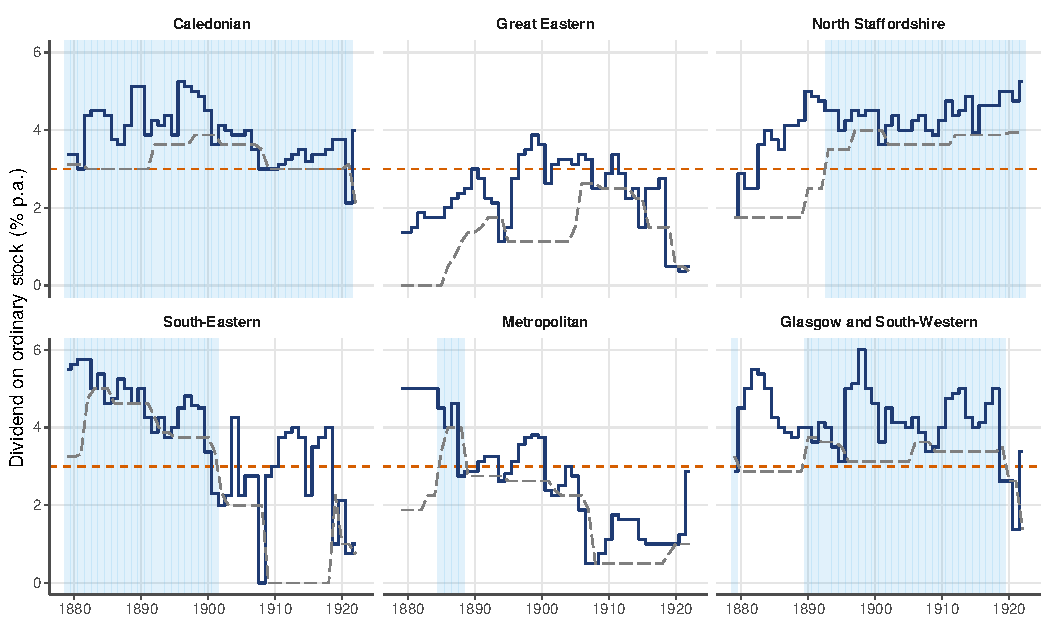
\includegraphics[width=\textwidth]{../output/exhibits/figures/fig1_dividend_histories.pdf}
\caption{Ordinary dividends and trustee eligibility, six companies. Solid line: annual dividend on ordinary stock. Dashed grey line: minimum over the previous ten years. Dashed orange line: the 3\% threshold. Shading: years in which the company's senior stocks were trustee-eligible.}\label{fig:histories}
\end{figure}

\begin{figure}[p]\centering
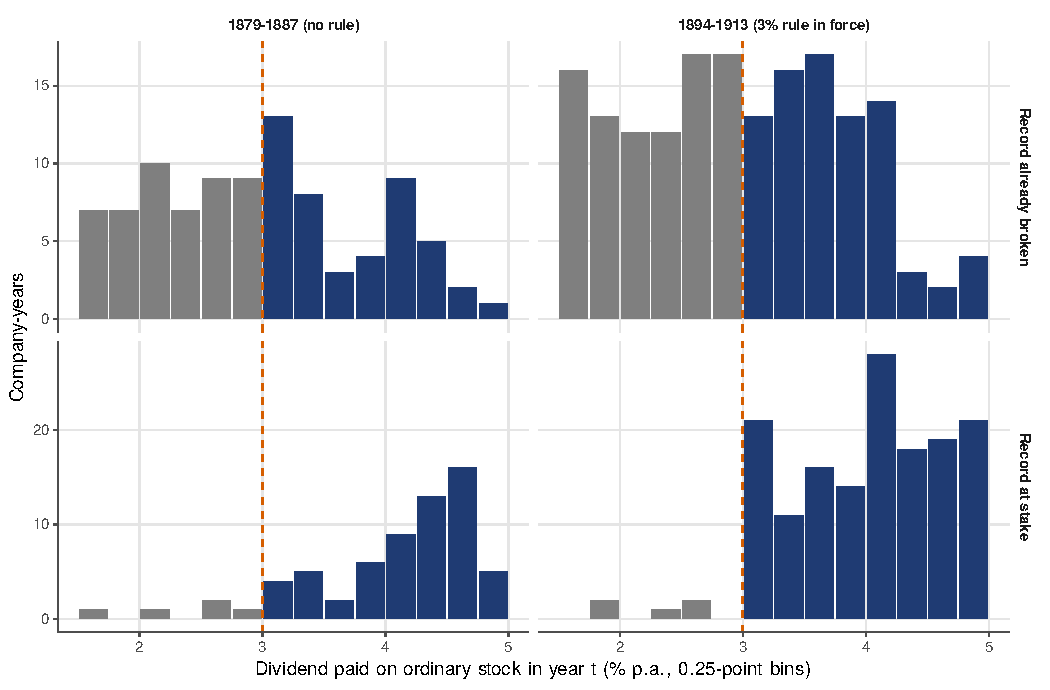
\includegraphics[width=\textwidth]{../output/exhibits/figures/fig2_dividend_bunching.pdf}
\caption{Dividend bunching at the threshold. Company-years by annual ordinary dividend (0.25-point bins). ``Record at stake'': the company paid at least 3\% in each of the previous nine years, so a lower dividend this year breaks a ten-year record.}\label{fig:bunching}
\end{figure}

\begin{figure}[p]\centering
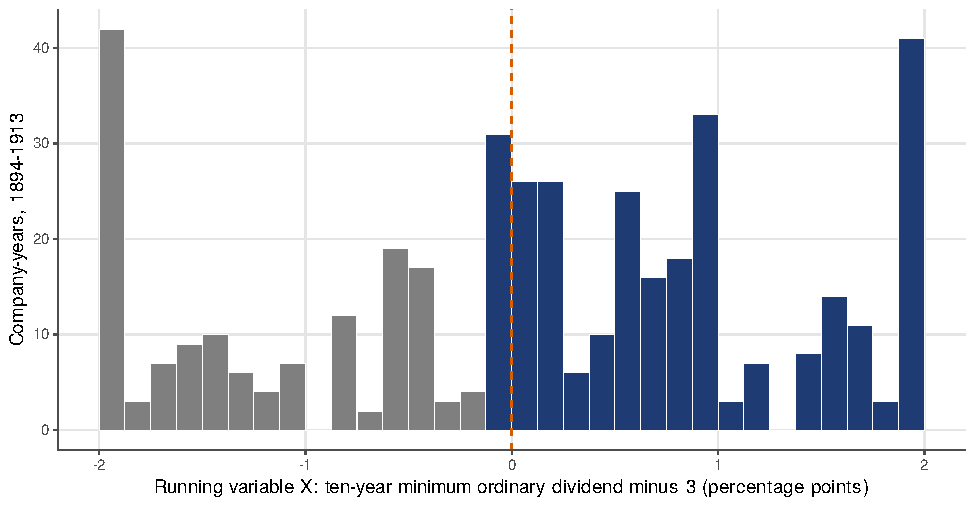
\includegraphics[width=0.9\textwidth]{../output/exhibits/figures/fig3_running_variable.pdf}
\caption{Distribution of the running variable, company-years 1894--1913. The spike at $X = 0$ is companies whose ten-year minimum is exactly 3.00\%.}\label{fig:rv}
\end{figure}

\begin{figure}[p]\centering
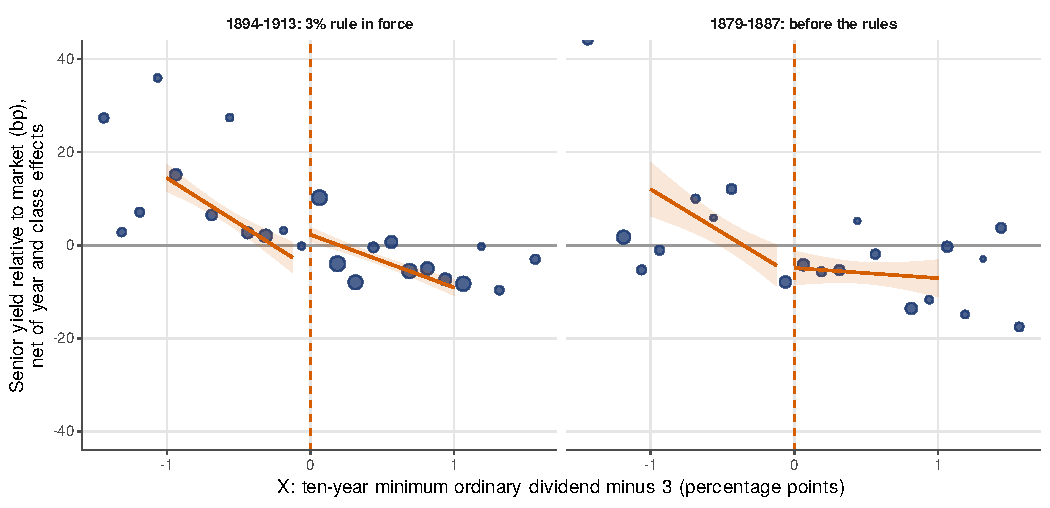
\includegraphics[width=\textwidth]{../output/results/figures/fig5_rd_plot.pdf}
\caption{Senior yields at the eligibility threshold. Points: mean yield relative to market, net of year and security-class effects, in 0.125-point bins of $X$ (size proportional to observations). Lines: separate linear fits within one point of the threshold, with 95\% confidence bands.}\label{fig:rd}
\end{figure}

\begin{figure}[p]\centering
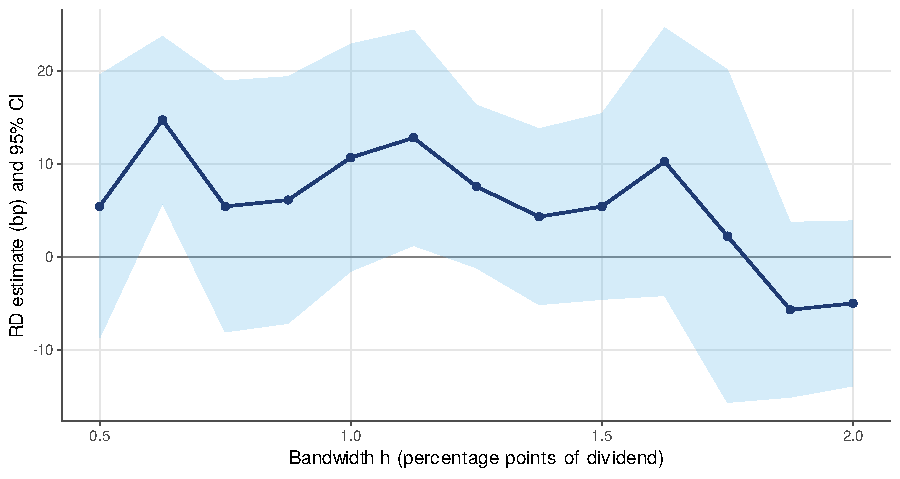
\includegraphics[width=0.85\textwidth]{../output/results/figures/fig6_bandwidth.pdf}
\caption{Bandwidth sensitivity. Local linear RD estimates (1894--1913) and 95\% confidence intervals clustered by company.}\label{fig:bandwidth}
\end{figure}

\begin{figure}[p]\centering
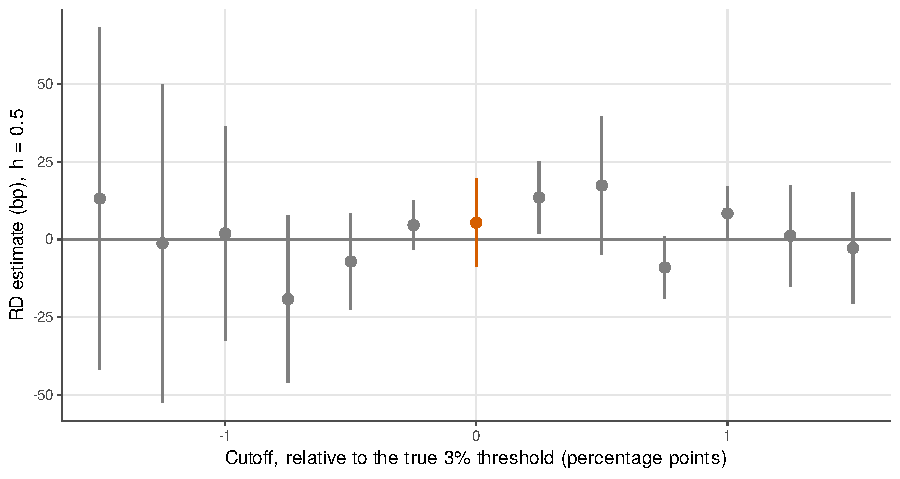
\includegraphics[width=0.85\textwidth]{../output/results/figures/fig7_placebo_cutoffs.pdf}
\caption{Placebo cutoffs. RD estimates ($h = 0.5$) at false thresholds, each using only observations on one side of the true threshold; the true threshold is highlighted.}\label{fig:placebo}
\end{figure}

\begin{figure}[p]\centering
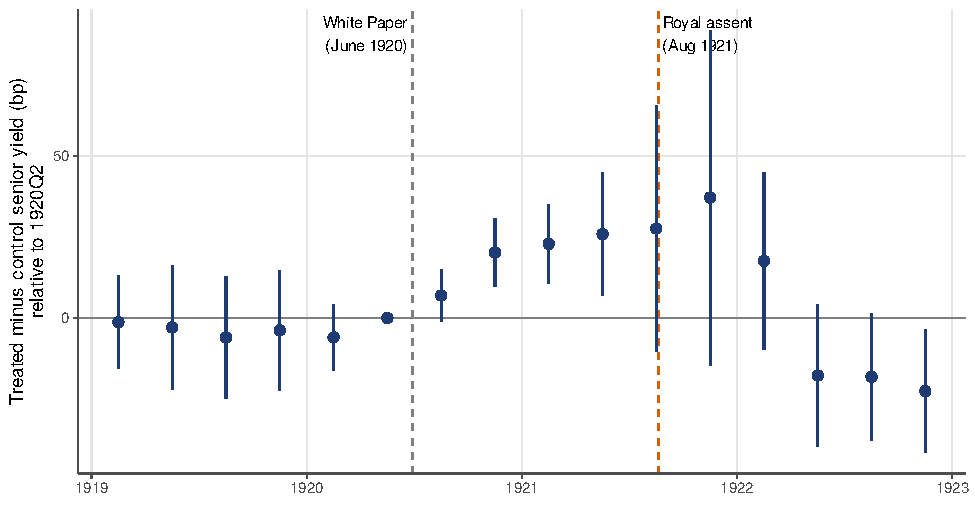
\includegraphics[width=0.9\textwidth]{../output/results/figures/fig8_event_study.pdf}
\caption{The Railways Act 1921: event study. Quarterly differences in senior yields between amalgamated companies that gained trustee status only through s.15 and those that already qualified, relative to 1920Q2, with security and month fixed effects and 95\% intervals clustered by company.}\label{fig:event}
\end{figure}

\begin{figure}[p]\centering
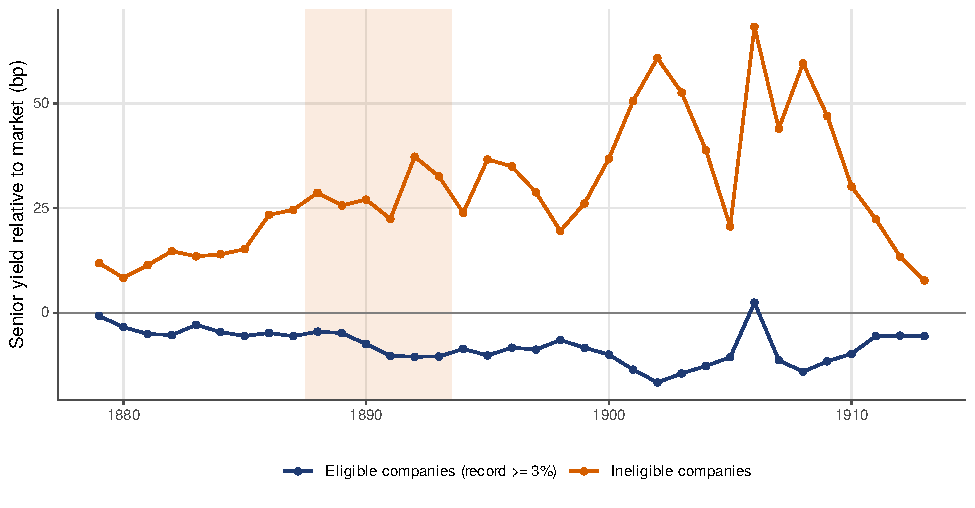
\includegraphics[width=0.9\textwidth]{../output/exhibits/figures/fig4_yield_gap.pdf}
\caption{Senior yields of eligible and ineligible companies, 1879--1913. Annual means of yields relative to market. Shading: the 1888--1893 reforms.}\label{fig:gap}
\end{figure}

\end{document}
